%!TeX program = xelatex
\documentclass[12pt,a4paper,UTF8]{ctexart}
\usepackage{zjureport}

\newcolumntype{Y}{>{\raggedright\arraybackslash}X}
\newcommand{\code}[1]{\texttt{#1}}
\newcommand{\twolinecode}[2]{\begin{tabular}[t]{@{}l@{}}\code{#1}\\\code{#2}\end{tabular}}
\newcommand{\sourcefile}[1]{\path{#1}}
\setlength{\parskip}{0.35em}
\setlength{\parindent}{2em}
\emergencystretch=3em
\sloppy

%%-------------------------------正文开始---------------------------%%
\begin{document}
\sloppy

%%-----------------------封面--------------------%%
\cover
\clearpage

%%------------------摘要-------------%%
\pagenumbering{Roman}
\thispagestyle{empty}
\clearpage
\begin{abstract}
转座元件（transposable elements, TEs）构成人类基因组的重要重复序列组成部分，并参与基因调控、遗传变异、肿瘤和人类遗传疾病等多个研究问题。TE 相关证据分散在文献、分类体系、表达矩阵和疾病/功能实体之间，单独依赖文献列表或表达矩阵都难以解释“某个 TE 与哪些疾病、机制、文献和表达背景有关”。TE-KG 因此定位为一个面向人类 TEs 的知识图谱数据库和浏览系统。当前系统不是单一表格或单一网页，而是由 Neo4j 图数据库、MySQL 表达摘要库、PHP API、浏览器 G6 图谱工作区、TE taxonomy 文件资源、PubMed 元数据和 2025 年期刊指标映射共同组成的数据库应用。本报告以仓库当前文档、代码和只读检查结果为事实来源，系统说明 TE-KG 的设计目标、运行架构、数据模型、核心实体与关系、证据支持层、表达数据层、前端检索与可视化能力、可靠性检查、已知边界和后续维护重点。

截至本报告检查时，TE-KG 的 Neo4j runtime target 为 \code{tekg3}。首页统计 API 与直接 Neo4j 检查确认当前运行时包含 11,415 个节点和 13,696 条有向关系，其中包括 12,444 条 \code{BIO\_RELATION}、2,308 个 \code{Paper} 节点和 225 个 \code{TE} 节点。PubMed 证据层已覆盖 2,308 个唯一 PMID，并已完成 2,308 条 PubMed metadata 记录抓取，失败数为 0。2025 年期刊影响因子元数据已映射到 2,037 个 \code{Paper} 节点，271 个 \code{Paper} 节点保持 null/unmatched。表达数据运行时根目录为 \sourcefile{data/bulk_expression_web}，包含 37,868 个 TE expression rows，并组织为 normal tissue、normal cell line 和 cancer cell line 三类数据集。报告最后专门说明数据获取流程的当前状态：\sourcefile{scripts/data_resource_update.py} 可作为 PubMed 检索、摘要抓取、LLM 信息抽取和 TE 白名单过滤的初版参考，但其数据获取模块仍由另一位负责人维护，尚不应作为最终 canonical pipeline 描述。
\end{abstract}

\clearpage

%%--------------------------目录页------------------------%%
\clearpage
\tableofcontents

%%------------------------正文页从这里开始-------------------%
\clearpage
\pagenumbering{arabic}

\section{报告范围与事实来源}

本报告的目标是把 TE-KG 数据库解释清楚：它存储什么、怎么存、哪些页面和 API 消费这些数据、哪些功能已经验证、哪些部分仍有边界。为了避免把历史聊天或未验证推断写入报告，本文只采用以下来源：

\begin{itemize}
  \item 仓库架构文档：\sourcefile{ARCHITECTURE.md}、\sourcefile{docs/architecture/current_system.md}、\sourcefile{docs/architecture/data_sources.md}、\sourcefile{docs/architecture/database_contract.md} 等\cite{tekg_architecture_entry,tekg_current_system,tekg_data_sources,tekg_database_contract}。
  \item 可靠性与完成计划：\sourcefile{docs/RELIABILITY.md}、PubMed metadata、journal metrics、relation aggregation、G6 evidence UX、TE tree load regression 等完成计划\cite{tekg_reliability,tekg_pubmed_metadata_v2,tekg_journal_metrics_import,tekg_relation_aggregation,tekg_g6_evidence,tekg_g6_tree}。
  \item 只读检查命令结果包括以下脚本：
  \begin{itemize}
    \item \code{check\_home\_stats\_api.py}
    \item \code{check\_neo4j\_tekg3.py}
    \item \code{check\_api\_contracts.py}
    \item \code{check\_expression\_paths.py}
    \item \code{check\_journal\_metrics\_neo4j\_import.py}
    \item \code{check\_relation\_journal\_metrics\_aggregation.py}
    \item \code{check\_graph\_api\_evidence\_support.py}
    \item \code{check\_graph\_api\_edge\_evidence\_records.py}
    \item \code{check\_g6\_te\_tree\_load\_regression.py}
  \end{itemize}
  \item 运行时代码入口：PHP root pages、\sourcefile{api/graph.php}、\sourcefile{api/graph_service.php}、\sourcefile{api/taxonomy.php}、\sourcefile{api/home_stats.php}、\sourcefile{api/expression_repository.php}、\sourcefile{path_config.php} 和 G6 前端文件。
  \item 数据获取初版脚本：\sourcefile{scripts/data_resource_update.py}。该脚本只用于说明数据获取思路，不用于给出最终采集质量结论。
\end{itemize}

本文不把 Impact Factor 写成 relation confidence，不把 \code{support\_*} 字段解释为置信度，不补推缺失影响因子。凡是缺失、未匹配或未验证的数据，均保持 null、unknown 或 unmatched 的语义。

\section{科学背景与资源问题}

TE-KG 需要解决的首要问题不是“如何展示一个更复杂的网页”，而是如何把分散的 TE 研究证据组织为可以追踪来源、可以按实体浏览、可以按表达背景补充解释的数据库资源。人类基因组初始测序工作已经显示，重复序列和转座元件是理解基因组结构、演化和功能的重要组成部分\cite{lander_human_genome_2001}。后续研究进一步表明，TE 插入、保留、调控和异常表达与人类遗传疾病和癌症存在多层关联\cite{payer_burns_te_disease_2019,burns_te_cancer_2017}。在功能层面，内源性逆转录病毒等 TE 片段还可被宿主调控网络 co-option，例如参与先天免疫相关基因调控\cite{chuong_erv_immunity_2016}。在表达层面，TE-derived reads 容易被常规转录组流程丢弃或误解释，因此 TE 表达分析需要专门的数据处理和解释边界\cite{lanciano_te_expression_2020}。

这些背景决定了 TE-KG 的资源价值：用户需要在同一个系统中同时看到 TE 名称和 taxonomy、TE--疾病/功能/基因等图谱关系、支撑每条关系的 PMID-level evidence、文献元数据、期刊指标的匹配状态，以及不同组织和细胞系背景下的表达摘要。TE-KG 目前实现的是一个本地、可审计的 pilot resource，而不是已经完成公开发布的权威数据库。它的边界也必须写清楚：图谱边表示从文献和导入流程中组织出的 evidence-supported relationship，不等于因果证明；\code{support\_*} 字段表示证据数量和期刊指标覆盖情况，不等于统计置信度；缺失影响因子、未匹配期刊和未覆盖数据均保持 null、unknown 或 unmatched。

从开放数据角度看，TE-KG 的长期目标应与 FAIR 数据原则保持一致，即让数据和元数据尽可能可发现、可访问、可互操作和可复用\cite{wilkinson_fair_2016}。但本报告只描述当前仓库已经实现和已验证的能力，不把尚未完成的公开部署、数据下载规范、许可证、DOI 或正式 repository accession 写成既成事实。

\section{系统定位与核心贡献}

TE-KG 的定位是一个转座元件知识图谱数据库和浏览系统。它把 TE、疾病、功能、基因、蛋白、RNA、突变、药物、毒素、脂类、肽类、糖类和文献等异质对象组织为可查询图谱，并在图谱边上保留 PMID-level 文献证据。系统同时提供表达数据浏览页面，使用户能够从 TE 名称进入不同组织、正常细胞系和癌细胞系的表达摘要。换言之，TE-KG 不是单纯的“文献列表”，也不是单纯的“表达矩阵查看器”，而是一个以图数据库为核心、以证据追踪为重点的多层数据库应用。

按照 resource/database report 的写作逻辑，TE-KG 当前已经形成三项核心贡献。第一，它把 TE-centered biomedical entities 组织为 Neo4j 图谱，并用统一 API 向页面和 G6 工作区提供查询结果。第二，它把 PubMed metadata、2025 年期刊指标映射和 relation-level support aggregation 接入图谱边，使用户能够从关系直接回到 PMID 证据。第三，它把表达数据整理为 MySQL summary tables，并通过 expression browse/detail 页面提供可分页、可排序、可按 context 解释的表达摘要。这三项贡献都以本报告后续章节列出的仓库检查和完成计划为依据。

当前运行形态为本地 PHP + browser JavaScript + Neo4j + MySQL。WAMP 提供 PHP runtime，Neo4j 的当前 runtime database 为 \code{tekg3}，MySQL 主要支撑 expression summary tables。前端页面仍位于项目根目录，包括 \sourcefile{index.php}、\sourcefile{browse.php}、\sourcefile{preview.php}、\sourcefile{path_finder.php}、\sourcefile{expression.php} 和 \sourcefile{expression_detail.php}。路径抽象由 \sourcefile{path_config.php}、\sourcefile{assets/js/tekg_paths.php} 和 \sourcefile{scripts/path_helpers.py} 分别服务 PHP、浏览器 JavaScript 和 Python 脚本。

\begin{figure}[H]
  \centering
  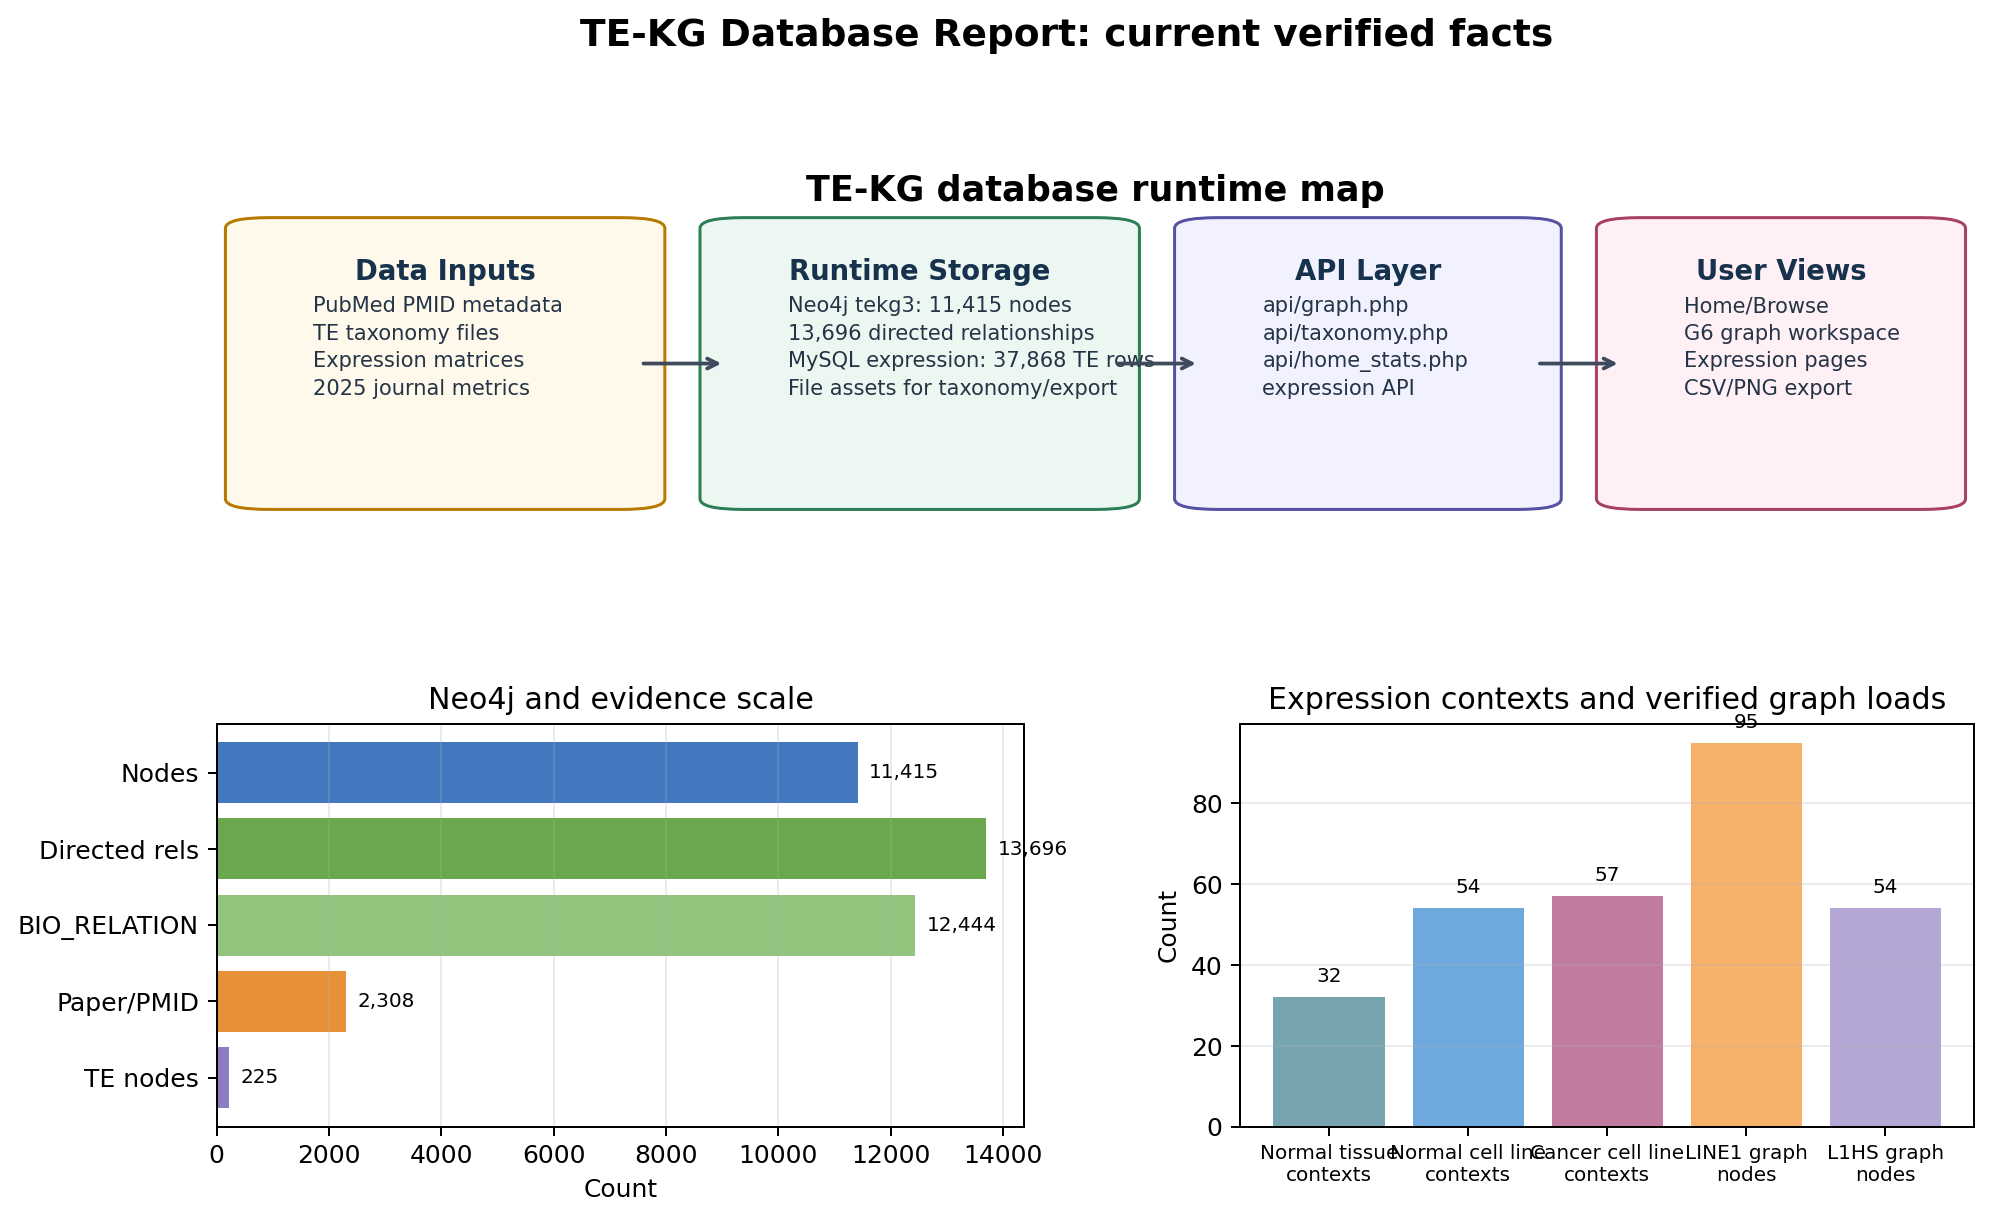
\includegraphics[width=\textwidth]{figures/tekg_database_overview.png}
  \caption{TE-KG 当前数据库运行时和已验证规模概览。图中数据来自本报告执行的只读检查、仓库完成计划和 docs/homework/tekg\_database\_report\_data.csv。}
  \label{fig:database-overview}
\end{figure}

\section{总体架构}

\subsection{分层架构}

TE-KG 可以分为六层：

\begin{enumerate}
  \item 数据输入层：包括 PubMed PMID / metadata、TE taxonomy 文件、expression matrices、2025 年期刊指标包、历史导入材料和处理后文件。
  \item 持久化层：Neo4j \code{tekg3} 存储知识图谱主体；MySQL \code{tekg\_expression} 存储表达摘要；文件系统保存 taxonomy、JBrowse、processed JSONL/TSV、导出源数据和缓存。
  \item API 层：\sourcefile{api/graph.php}、\sourcefile{api/taxonomy.php}、\sourcefile{api/home_stats.php}、\sourcefile{api/health.php}、\sourcefile{api/te_metrics.php}、expression repository 等向页面提供统一 JSON 或 PHP 数据接口。
  \item 页面层：根目录 PHP 页面负责页面结构、表单、导航、筛选控件和数据展示容器。
  \item 图谱渲染层：\sourcefile{assets/js/renderers/g6/} 内的 G6 runtime 负责动态子图、TE taxonomy tree、图例筛选、节点/边 inspect card、evidence table 和导出。
  \item 可靠性层：\sourcefile{scripts/checks/} 中的检查脚本验证数据库配置、API contract、taxonomy runtime truth、expression path、G6 browser smoke、journal metrics 和 relation support 聚合。
\end{enumerate}

该架构的关键原则是：Neo4j/API 是 TE taxonomy 和知识图谱 runtime truth source；expression runtime 根目录是 \sourcefile{data/bulk_expression_web}；旧数据库 \code{tekg2}/\code{tekg21} 不应作为 fallback 回流；缺少本地配置时应显式报错，而不是静默切换到旧库。

\subsection{核心运行入口}

\begin{longtable}{p{0.26\textwidth}p{0.28\textwidth}p{0.38\textwidth}}
\caption{TE-KG 当前主要入口与职责}\\
\toprule
入口 & 类型 & 职责 \\
\midrule
\endfirsthead
\toprule
入口 & 类型 & 职责 \\
\midrule
\endhead
\sourcefile{index.php} & 首页 & 展示数据库总览、入口卡片、统计图和数据资源状态。首页统计应优先来自轻量 API 或缓存。 \\
\sourcefile{browse.php} & TE browse 页面 & 面向 TE 条目的浏览、筛选和跳转。当前仍是 TE-oriented 页面，不扩展为全实体搜索页。 \\
\sourcefile{preview.php} & 图谱工作区 & G6 / TE-KG graph workspace，支持搜索、树图、动态图、节点/边 inspect card、evidence support 和导出。 \\
\sourcefile{path_finder.php} & 路径查找页面 & 面向实体关系路径的探索入口。 \\
\sourcefile{expression.php} & 表达浏览页面 & 基于 MySQL expression summary tables 浏览 TE expression top contexts、排序、筛选和分页。 \\
\sourcefile{expression_detail.php} & 表达详情页面 & 展示单个 TE 在不同 expression datasets 和 contexts 下的统计摘要与图表。 \\
\sourcefile{api/graph.php} & 图谱 API & 接收 \code{q}、\code{type}、\code{class}、\code{key\_level} 和 expand 参数，返回 anchor、matches、elements 和 evidence fields。 \\
\sourcefile{api/taxonomy.php} & Taxonomy API & 返回 file tree taxonomy payload 或 Neo4j-backed taxonomy items/summary。 \\
\sourcefile{api/home_stats.php} & 统计 API & 从 Neo4j \code{tekg3} 返回总节点、总关系、实体构成、关系构成和 TE 分类构成。 \\
\sourcefile{api/expression_repository.php} & Expression repository & 连接 MySQL，读取 expression context catalog、browse summary、dataset summary 和 context stats。 \\
\bottomrule
\end{longtable}

\section{数据库规模与数据模型}

\subsection{Neo4j 运行时规模}

本报告采用 \sourcefile{api/home_stats.php} 与 \code{check\_home\_stats\_api.py} 的口径作为 Neo4j runtime 总规模口径：11,415 个节点、13,696 条有向关系。完成计划中的结构证据显示，这 13,696 条有向关系由 12,444 条 \code{BIO\_RELATION}、744 条 \code{HAS\_SUBCATEGORY}、436 条 \code{CLASSIFIED\_AS} 和 72 条 \code{SUBFAMILY\_OF} 组成。另一个检查脚本 \code{check\_neo4j\_tekg3.py} 输出 24,748 个 \code{BIO\_RELATION} 相关计数；该数值来自该脚本自身的查询口径，不作为数据库关系总数使用。为了避免混淆，本文所有总节点/总关系规模均以 \code{home\_stats} 和结构证据为准。

\begin{table}[H]
  \centering
  \caption{Neo4j \code{tekg3} 主要规模口径}
  \begin{tabularx}{\textwidth}{l r Y}
    \toprule
    指标 & 数值 & 说明 \\
    \midrule
    总节点 & 11,415 & \code{MATCH (n) RETURN count(n)}，由 home stats API 验证。 \\
    总有向关系 & 13,696 & \code{MATCH ()-[r]->() RETURN count(r)}，由 home stats API 验证。 \\
    \code{BIO\_RELATION} & 12,444 & 文献/实体关系主体，已完成 relation support 聚合。 \\
    \code{HAS\_SUBCATEGORY} & 744 & 疾病分类层级关系。 \\
    \code{CLASSIFIED\_AS} & 436 & 疾病到分类节点的归属关系。 \\
    \code{SUBFAMILY\_OF} & 72 & TE taxonomy 层级中的 subfamily 关系。 \\
    TE 节点 & 225 & \code{check\_neo4j\_tekg3.py} 验证，并可解析 AluJb、L1HS、SVA。 \\
    Paper 节点 & 2,308 & 每个节点含非空 \code{pmid}，与 PubMed metadata 记录一一对应。 \\
    \bottomrule
  \end{tabularx}
\end{table}

\subsection{实体类型构成}

当前 Neo4j 节点使用 label 表达实体类型。节点类型和数量如下表。Function 和 Paper 是数量最大的两类，分别用于表示机制/过程实体和文献证据锚点。TE 节点虽然只有 225 个，但它们是图谱的中心入口之一，很多搜索和图谱展开都以 TE 名称或 TE alias 为中心。

\begin{longtable}{l r r p{0.48\textwidth}}
\caption{Neo4j 节点 label 构成}\\
\toprule
Label & 数量 & 占比 & 说明 \\
\midrule
\endfirsthead
\toprule
Label & 数量 & 占比 & 说明 \\
\midrule
\endhead
Function & 3,683 & 32.26\% & 生物过程、机制、功能或抽象事件。 \\
Paper & 2,308 & 20.22\% & 文献节点，当前通过 \code{pmid} 与 \code{BIO\_RELATION.pmids} 连接。 \\
Gene & 1,280 & 11.21\% & 非 TE 基因实体。 \\
Protein & 1,089 & 9.54\% & 蛋白实体。 \\
DiseaseCategory & 767 & 6.72\% & 疾病分类层级节点。 \\
Disease & 676 & 5.92\% & 疾病实体。 \\
RNA & 588 & 5.15\% & mRNA、lncRNA、miRNA 等 RNA 实体。 \\
Mutation & 377 & 3.30\% & 插入、突变或变异事件。 \\
Pharmaceutical & 293 & 2.57\% & 药物、化合物或候选药物。 \\
TE & 225 & 1.97\% & 转座元件实体。 \\
Toxin & 67 & 0.59\% & 毒素实体。 \\
Lipid & 26 & 0.23\% & 脂类实体。 \\
Peptide & 23 & 0.20\% & 肽类实体。 \\
Carbohydrate & 12 & 0.11\% & 糖类实体。 \\
NonHumanTE & 1 & 0.01\% & 非人类 TE 标记。 \\
\bottomrule
\end{longtable}

\subsection{关系类型与谓词}

Neo4j 关系类型分为两层：第一层是关系 type，例如 \code{BIO\_RELATION}、\code{HAS\_SUBCATEGORY}、\code{CLASSIFIED\_AS} 和 \code{SUBFAMILY\_OF}；第二层是 \code{BIO\_RELATION.predicate}，例如 \code{regulate}、\code{lead to}、\code{express}、\code{inhibit}、\code{affect} 等。首页统计 API 为了展示更具信息量的关系构成，会过滤掉非常宽泛的 \code{associate with}、\code{participate in} 和 \code{involve in}，然后显示具体谓词 Top 5 和 Other。因此，首页的 relation composition 总数低于 12,444 条 \code{BIO\_RELATION} 总数，这是展示口径差异，不是数据丢失。

\begin{table}[H]
  \centering
  \caption{首页统计 API 中的具体关系谓词构成}
  \begin{tabularx}{0.9\textwidth}{l r r Y}
    \toprule
    谓词 & 数量 & 占比 & 说明 \\
    \midrule
    regulate & 717 & 9.02\% & 调控关系。 \\
    lead to & 659 & 8.29\% & 导致或引发关系。 \\
    express & 612 & 7.70\% & 表达关系。 \\
    inhibit & 589 & 7.41\% & 抑制关系。 \\
    affect & 546 & 6.87\% & 影响关系。 \\
    Other & 4,825 & 60.71\% & 过滤宽泛谓词后其余具体谓词合并。 \\
    \bottomrule
  \end{tabularx}
\end{table}

\section{TE taxonomy 层}

TE taxonomy 是 TE-KG 的核心组织维度之一。当前 canonical runtime 规则是：TE taxonomy 以 Neo4j/API 为准，历史文件可以作为 reference 或构建输入，但不能重新成为页面 runtime truth source。系统同时保留 file tree taxonomy API，用于 G6 TE tree 展示。

\subsection{当前 taxonomy 数据}

\code{api/taxonomy.php?view=tree\&source=rmsk\_repbase} 返回 file tree payload。G6 TE tree load regression 检查确认当前 taxonomy tree 包含 1,632 个节点和 1,631 条边。该检查还确认 L1HS 路径已经恢复：

\tbox{
TE - Human $\rightarrow$ Class I: Retrotransposons $\rightarrow$ Order: Non-LTR Retrotransposons (LINEs) $\rightarrow$ Superfamily: L1 (LINE-1) $\rightarrow$ Family: L1PA $\rightarrow$ L1HS
}

首页 TE classification composition 的默认 \code{class} 口径只统计满足 \code{homepage\_chart\_included=true}、\code{taxonomy\_source=tree\_rmsk\_repbase} 且 \code{taxonomy\_class} 非空的 TE 节点。因此，首页分类图中的 TE 数量不是全部 225 个 TE 节点，而是该展示口径下的 154 个 TE：Retrotransposons 127 个，占 82.47\%；DNA Transposons 27 个，占 17.53\%。

\subsection{已知 taxonomy 风险}

当前两个 taxonomy 检查仍提示首页 ring chart 尚未完全加载 \sourcefile{api/taxonomy_lib.php} 或完全从 realtime Neo4j taxonomy 构建视图：
\code{check\_taxonomy\_runtime\_truth.py} 和 \code{check\_taxonomy\_runtime\_consistency.py}。
因此，报告中必须区分：

\begin{itemize}
  \item \code{api/taxonomy.php} 和 G6 TE tree 的 taxonomy API/树图路径已经有检查覆盖。
  \item 首页 ring chart 是数据入口和展示组件，但其 canonical source 对齐仍是技术债。
  \item 不能把首页 ring chart 作为“全系统 taxonomy 已完全 canonical”的证据。
\end{itemize}

\section{PubMed 文献证据层}

\subsection{Paper 节点与 PMID}

TE-KG 当前不新建独立 Publication/Article/Evidence label，而是复用已有 \code{Paper} 节点作为文献证据锚点。每个 \code{Paper} 节点含 \code{pmid} 属性，\code{BIO\_RELATION} 关系含 \code{pmids} 数组。两者通过 PMID 连接：\code{BIO\_RELATION.pmids -> Paper.pmid}。该设计避免了为关系再创建平行证据图模型，也避免了 Neo4j relationship 无法直接连接 relationship 的建模问题。

PubMed metadata enrichment v2 已完成完整抓取：2,308 个唯一 PMID，2,308 条 metadata records，0 个失败。完整输出 sanity check 通过，字段覆盖如下：

\begin{table}[H]
  \centering
  \caption{PubMed metadata 字段覆盖}
  \begin{tabularx}{0.86\textwidth}{l r Y}
    \toprule
    字段或信息 & 覆盖数量 & 说明 \\
    \midrule
    PMID metadata records & 2,308 & 与 Neo4j \code{Paper.pmid} 对齐。 \\
    DOI & 2,244 & PubMed metadata 中可解析 DOI 的记录数。 \\
    Journal & 2,308 & 每条记录均有 journal 信息。 \\
    Year & 2,308 & 每条记录均有发表年份。 \\
    Authors & 2,307 & 仅 1 条记录缺少作者字段。 \\
    MeSH terms & 2,087 & 包含 MeSH term 的记录数。 \\
    Keywords & 827 & 包含关键词的记录数。 \\
    Grants & 1,064 & 包含 grant/funding 信息的记录数。 \\
    Chemicals & 1,888 & 包含 chemical list 的记录数。 \\
    References & 1,607 & 包含 reference list 的记录数。 \\
    \bottomrule
  \end{tabularx}
\end{table}

PubMed XML 不提供 Impact Factor。因此，PubMed metadata 只提供文献事实字段，如 PMID、DOI、标题、摘要可用性、期刊、年份、作者、MeSH、关键词、基金、化学物质和引用。影响因子必须来自外部期刊指标映射，不能由 PubMed 或 LLM 推断。

\subsection{2025 年期刊指标映射}

TE-KG 当前采用 2025 年期刊影响因子元数据作为期刊层面辅助信息。该数据源在项目内以 \code{impact\_factor\_package\_2025} 表示，不能表述为官方 JCR direct export。映射结果如下：

\begin{itemize}
  \item unique journal rows：686。
  \item matched journals：594；unmatched journals：92。
  \item PMID total：2,308。
  \item PMID matched：2,037；PMID unmatched：271。
  \item eISSN match：435；print ISSN match：137；title exact fallback：22。
  \item JCR quartile coverage：594；CAS partition coverage：318。
\end{itemize}

映射到 Neo4j 后，2,308 个 \code{Paper} 节点均带有 journal metrics import tag，其中 2,037 个节点有非空 \code{journal\_metric\_value}，271 个节点保持 null metric values。缺失值不能填 0，不能被模型补全，也不能被解释为低影响因子。

\section{BIO\_RELATION 证据支持聚合}

\subsection{聚合设计}

Relation support 聚合以 \code{BIO\_RELATION.pmids} 为输入，通过 \code{Paper.pmid} 查找文献元数据和 2025 期刊指标，然后把派生统计写回已有 \code{BIO\_RELATION} 关系。这个过程只写属性，不创建或删除节点/关系，不改变图谱拓扑，不修改 taxonomy、agent 或 expression 模块。

写入字段包括：

\begin{itemize}
  \item \code{support\_pmid\_count}：关系支持 PMID 去重计数。
  \item \code{support\_metric\_paper\_count}：支持 PMID 中有非空期刊指标的记录数。
  \item \code{support\_metric\_coverage}：有指标 PMID 数 / 支持 PMID 数。
  \item \code{support\_if\_max}、\code{support\_if\_mean}、\code{support\_if\_median}：只对非空 IF 值聚合。
  \item \code{support\_jcr\_q1\_count} 到 \code{support\_jcr\_q4\_count}：JCR quartile 计数。
  \item \code{support\_journal\_count}：支持文献涉及的非空 journal title 数。
  \item \code{support\_publication\_year\_min}、\code{support\_publication\_year\_max}：支持文献年份范围。
  \item \code{relation\_metrics\_import\_tag}：当前 tag 为 \code{relation\_metrics\_v1\_2026-05-22}。
\end{itemize}

这些字段只能解释为 evidence support，不是 confidence。期刊指标用于辅助文献元数据展示，不证明 TE--疾病或 TE--功能关系为因果关系。

\subsection{聚合结果}

当前 relation aggregation 检查通过，确认 12,444/12,444 条 \code{BIO\_RELATION} 已带有聚合标签，且没有非 \code{BIO\_RELATION} 关系被污染。聚合 dry-run/write 证据如下：

\begin{table}[H]
  \centering
  \caption{BIO\_RELATION relation support 聚合结果}
  \begin{tabularx}{\textwidth}{l r Y}
    \toprule
    指标 & 数值 & 说明 \\
    \midrule
    \code{BIO\_RELATION} total & 12,444 & 现有 directed \code{BIO\_RELATION}。 \\
    with pmids & 12,444 & 当前所有 \code{BIO\_RELATION} 均有非空 PMID 数组。 \\
    raw PMID references & 14,770 & 未去重前 relation PMID 引用数。 \\
    unique relation PMIDs & 2,270 & relation 侧去重 PMID 数。 \\
    joinable PMIDs & 2,270 & 能与 \code{Paper.pmid} 连接的 PMID 数。 \\
    PMIDs with metric & 2,003 & relation 侧 PMID 中带 2025 指标的数量。 \\
    PMIDs without metric & 267 & relation 侧 PMID 中未匹配指标的数量。 \\
    updated relations & 12,444 & 写入 support 聚合属性的关系数。 \\
    \bottomrule
  \end{tabularx}
\end{table}

支持 PMID 数分布为：1 篇支持文献的关系 11,705 条；2 篇支持文献的关系 434 条；3--5 篇支持文献的关系 219 条；6--10 篇支持文献的关系 53 条；超过 10 篇支持文献的关系 33 条。metric coverage 分布为：0 覆盖 1,354 条，(0.25, 0.5] 覆盖 103 条，(0.5, 0.75] 覆盖 53 条，(0.75, 1) 覆盖 62 条，完全覆盖 10,872 条。

\section{Graph API 与 G6 图谱工作区}

\subsection{Graph API contract}

\sourcefile{api/graph.php} 是图谱查询入口。默认查询为空时使用 \code{LINE1}。主要参数包括：

\begin{itemize}
  \item \code{q}：查询词，如 \code{LINE1}、\code{L1HS}、疾病名或功能名。
  \item \code{type} 与 \code{class}：用于 disease class 查询。
  \item \code{key\_level}：控制关键节点扩展层级，范围 1--10。
  \item \code{expand\_node\_id}、\code{expand\_node\_type}、\code{expand\_query}：用于 G6 node card 的同名实体安全扩展。
\end{itemize}

\sourcefile{api/graph_service.php} 负责解析 anchor、选择 Disease/DiseaseClass/Paper/普通实体上下文、扩展 key nodes、合并 taxonomy 信息、构建前端 elements，并将 support fields 和 evidence records 写入 edge payload。\code{check\_api\_contracts.py} 当前确认 \code{api/health.php}、\code{api/graph.php?q=LINE1}、same-label expand disambiguation、taxonomy file tree 和 taxonomy items contract 均通过。

\subsection{Evidence records}

G6 evidence support UX v1 使每条图谱边除了原有 \code{pmids} 和 \code{support\_*} 字段外，还包含 eager \code{evidence\_records}。该字段故意不携带摘要文本，只包含紧凑证据元数据：

\begin{itemize}
  \item \code{pmid}
  \item \code{pubmed\_url}
  \item \code{pubmed\_title}
  \item \code{pubmed\_journal\_title}
  \item \code{pubmed\_publication\_year}
  \item \code{journal\_metric\_value}
  \item \code{journal\_metric\_source}
  \item \code{journal\_metric\_year}
  \item \code{journal\_jcr\_quartile}
  \item \code{journal\_metric\_match\_method}
\end{itemize}

检查结果确认，\code{api/graph.php?q=LINE1} 至少有边带有 support fields；样例检查边包含 65 个 PMIDs，并可返回 evidence records。缺失 Paper metadata 时，系统仍可生成最小记录：PMID 与 PubMed URL 保留，其他字段为 null。

\subsection{G6 工作区功能}

\sourcefile{preview.php} 是当前图谱工作区。父页面负责查询栏、图例、工具栏和状态；iframe 内 G6 runner 负责实际图谱渲染。当前已验证功能包括：

\begin{itemize}
  \item LINE1 动态图加载：95 nodes / 103 edges。
  \item L1HS 动态图加载：54 nodes / 58 edges。
  \item Taxonomy tree：1,632 nodes / 1,631 edges。
  \item Edge width 映射到 \code{support\_pmid\_count}；edge opacity 映射到 \code{support\_metric\_coverage}，coverage 为 0 的边仍保持可见。
  \item 点击边后，在 edge inspect card 的 PubMed 区域显示 evidence table，列包括 PMID、Year、Journal、IF、JCR、Match、Title。
  \item evidence records 超过 10 行时，支持下载 selected-edge evidence CSV。
  \item 当前可见子图支持 nodes CSV、edges CSV 和 canvas PNG 导出。
  \item SVG 导出未实现，界面保留 disabled 的 \code{SVG Soon}，不能写成已完成。
\end{itemize}

G6 tree 和 category 行为也有明确边界：\code{Class I: Retrotransposons}、\code{Class II: DNA Transposons}、\code{Others} 等 category node 在 tree 中保持树模式；普通 dynamic graph 搜索这些 category label 当前可能返回 empty graph payload，这是未实现 category-centered graph contract，而不是 loader 卡住或 Neo4j 故障。

\section{Expression 数据层}

\subsection{运行时根目录}

Expression runtime 根目录是 \sourcefile{data/bulk_expression_web}。这是当前系统明确约束；旧路径 \sourcefile{data/raw/new_data/bulk_expression_web} 不能恢复为 runtime 根目录。需要注意的是，\sourcefile{data/bulk_expression_web/processed/expression_processing_manifest.json} 的 \code{source\_files} 和 \code{output\_files} 字段仍记录了当时处理来源或历史输出路径，这些路径用于解释数据加工来源，不代表当前页面运行时根目录。

\code{check\_expression\_paths.py} 当前输出：

\tbox{
PASS expression path consistency；canonical root: \sourcefile{D:/wamp64/www/TE-/data/bulk_expression_web}
}

\subsection{表达数据规模}

Expression 数据包含三类 dataset：normal tissue、normal cell line、cancer cell line。处理清单确认每类 dataset 均含 37,868 个 TE rows。具体规模如下：

\begin{table}[H]
  \centering
  \caption{Expression 数据处理规模}
  \begin{tabularx}{\textwidth}{l r r r r Y}
    \toprule
    Dataset & TE rows & Matrix columns & Runs used & Contexts & 说明 \\
    \midrule
    Normal tissue & 37,868 & 205 & 200 & 32 & metadata 371 rows；5 个 matrix runs 缺失；同一 context 的重复 runs 为 171。 \\
    Normal cell line & 37,868 & 307 & 307 & 54 & metadata 307 rows；无 missing matrix runs。 \\
    Cancer cell line & 37,868 & 646 & 646 & 57 & metadata 646 rows；输入矩阵不含显式 TE column，使用共享 TE 顺序假设。 \\
    \bottomrule
  \end{tabularx}
\end{table}

处理清单还明确两个重要假设：第一，\code{mean} 与 \code{average} 被视为同一指标；第二，输入使用 normalized count，因此页面和报告不应擅自标注为 TPM。

\subsection{MySQL summary tables}

Expression 页面主要依赖 MySQL summary tables，而不是每次直接读取数百 MB 的原始矩阵。当前 schema 设计包括四张核心表：

\begin{longtable}{p{0.30\textwidth}p{0.62\textwidth}}
\caption{Expression MySQL 表职责}\\
\toprule
表名 & 职责 \\
\midrule
\endfirsthead
\toprule
表名 & 职责 \\
\midrule
\endhead
\twolinecode{expression\_context}{\_catalog} & 记录 dataset、context label、context full name、context order 和 run count，用于构建筛选项和上下文目录。 \\
\twolinecode{expression\_dataset}{\_summary} & 每个 TE 在每个 dataset 下的汇总行，包含 top context、max/mean/median、CV、breadth 等指标。主键为 \code{te\_name + dataset\_key}。 \\
\twolinecode{expression\_context}{\_stats} & 每个 TE 在每个 dataset/context 下的统计行，包含 sample count、min、q1、median、q3、mean、max、std、cv。主键为 \code{te\_name + dataset\_key + context\_label}。 \\
\twolinecode{expression\_browse}{\_summary} & 面向 \sourcefile{expression.php} 的跨 dataset 汇总表，包含 global top context 和各 dataset 的可用性、top context、breadth 和 CV 字段。主键为 \code{te\_name}。 \\
\bottomrule
\end{longtable}

\sourcefile{api/expression_repository.php} 提供 MySQL 连接、dataset key 规范化、metric/sort 规范化、TE 名称解析、筛选项读取、分页浏览和详情 bundle 读取。浏览页支持 keyword、dataset、top context、minimum global median、排序、分页；详情页支持 metric、sort 和 bar/box chart 选择。

\section{首页、Browse 与统计展示}

\subsection{首页统计}

\sourcefile{api/home_stats.php} 从 Neo4j \code{tekg3} 读取总节点、总关系、实体构成、关系构成和 TE 分类构成。它在启动时要求解析到 \code{tekg3}，若配置不满足则返回错误。当前检查确认：

\begin{itemize}
  \item nodes total = 11,415。
  \item relationships total = 13,696。
  \item entity composition 有 15 类。
  \item relation composition 有 6 类，即 Top 5 + Other。
  \item 默认 \code{te\_level=class}，并支持 order、superfamily、family 级别查询。
\end{itemize}

首页统计 API 的价值在于提供轻量 dashboard 数据，不需要页面加载时执行复杂图谱查询。其已验证字段可以作为数据库概览来源；但是首页 ring chart 的 taxonomy canonical 对齐仍需单独处理，不能与 home stats API 混为一谈。

\subsection{Browse 页面}

Browse 当前仍是 TE-oriented 页面。它适合做 TE 条目目录、筛选、跳转和与图谱/表达页面联动的入口，不应在当前阶段扩展成全实体搜索页。报告不把 Browse 写成“全库万能检索”，因为当前架构文档明确要求 Browse 保持 TE-oriented。

\section{数据获取流程初版说明}

数据获取由另一位负责人负责，因此本节只根据 \sourcefile{scripts/data_resource_update.py} 写初版流程说明，不把它当作最终生产管线。

\subsection{脚本目标}

\sourcefile{scripts/data_resource_update.py} 的目标是从 PubMed 检索 human transposon 相关文献，抓取标题和摘要，调用 DeepSeek 模型进行生物医学信息抽取，并输出 TE knowledge graph update JSONL。脚本核心步骤如下：

\begin{enumerate}
  \item 读取 TE names whitelist：从分号分隔文件读取 TE 名称，生成原始名称、小写名称和正则表达式。
  \item PubMed 检索：使用 human transposon 相关检索式，并按年份分割检索，避免单次 PubMed 结果上限。
  \item NCBI efetch：按 batch 获取 PubMed XML，解析 PMID、标题和摘要。
  \item 预过滤：若标题和摘要中没有命中任一 TE 白名单名称，则跳过。
  \item LLM 信息抽取：调用 DeepSeek chat completions API，把单篇文献转为 JSON object，包括 entities 和 relations。
  \item 白名单后处理：只保留 whitelist 中的 transposon 实体，并移除指向被删除 TE 的关系。
  \item 漏提检查：如果 whitelist 正则在文本中命中但 LLM 未抽取，则写入 missing log。
  \item 断点续传：读取已输出 JSONL 和 skipped log，避免重复处理 PMID。
  \item 输出：成功结果写 JSONL；失败、跳过、漏提分别写日志。
\end{enumerate}

\subsection{当前配置和边界}

该脚本当前采用环境变量读取 \code{DEEPSEEK\_API\_KEY}、\code{DEEPSEEK\_API\_URL} 和 \code{DEEPSEEK\_MODEL}，这是正确方向。但仍存在几个不能在正式报告中忽略的边界：

\begin{itemize}
  \item TE names file、输出 JSONL 和日志路径仍是本地绝对路径，需要迁移到仓库相对路径或配置文件。
  \item 脚本把 PubMed 检索、NCBI fetch、LLM 抽取、过滤、日志和断点续传都放在一个文件中，后续应拆成可测试模块。
  \item LLM 抽取结果需要 schema validation、fixture tests 和人工抽样验证，不能直接等同于事实。
  \item PubMed metadata enrichment v2 已经提供更稳定的 metadata parser；未来应避免与该脚本形成第二套不一致 PubMed metadata truth source。
  \item 当前数据获取负责人尚未确认最终搜索式、TE whitelist 来源、错误处理策略、输出 schema 和再导入 Neo4j 的质量门禁。
\end{itemize}

因此，本报告把 \sourcefile{scripts/data_resource_update.py} 定位为“数据获取初版参考流程”，而不是 TE-KG 当前已验证数据库规模的依据。当前规模仍以 Neo4j、MySQL summary、processed metadata 和 checks 为准。

\section{可靠性与质量控制}

TE-KG 的可靠性策略是先用可运行检查确认事实，再修改页面或报告。当前核心 checks 覆盖以下方面：

\begin{longtable}{p{0.36\textwidth}p{0.56\textwidth}}
\caption{本报告使用或引用的可靠性检查}\\
\toprule
检查命令 & 验证内容 \\
\midrule
\endfirsthead
\toprule
检查命令 & 验证内容 \\
\midrule
\endhead
\code{check\_neo4j\_tekg3.py} & 配置解析到 \code{tekg3}、\code{RETURN 1} 可执行、TE 节点存在、AluJb/L1HS/SVA 可解析。 \\
\code{check\_home\_stats\_api.py} & 首页统计 API 的总节点/关系、实体构成、关系构成、TE 分类构成与直接 Neo4j 查询一致。 \\
\code{check\_api\_contracts.py} & health、graph、taxonomy 和 same-label expand disambiguation contract。 \\
\code{check\_expression\_paths.py} & expression runtime root 保持 \sourcefile{data/bulk_expression_web}。 \\
\twolinecode{check\_journal\_metrics}{\_full\_mapping.py} & 2025 journal metrics CSV、metadata JSONL 和 mapping report 一致。 \\
\twolinecode{check\_journal\_metrics}{\_neo4j\_import.py} & \code{Paper} enrichment tag、metric/null counts、非 Paper 节点污染检查。 \\
\twolinecode{check\_relation\_journal}{\_metrics\_aggregation.py} & \code{BIO\_RELATION} support aggregation count 与不变量。 \\
\twolinecode{check\_graph\_api}{\_evidence\_support.py} & Graph API edge support fields 类型、范围和存在性。 \\
\twolinecode{check\_graph\_api\_edge}{\_evidence\_records.py} & edge \code{evidence\_records} contract。 \\
\twolinecode{check\_g6\_te\_tree}{\_load\_regression.py} & LINE1/L1HS 动态图加载、taxonomy tree、category click、loader 分类和 L1HS path。 \\
\twolinecode{check\_no\_legacy}{\_db\_fallback.py} & 活跃文件中没有 \code{tekg2}/\code{tekg21} runtime fallback。 \\
\bottomrule
\end{longtable}

本报告执行时，有两个 taxonomy 检查仍失败：\code{check\_taxonomy\_runtime\_truth.py} 和 \code{check\_taxonomy\_runtime\_consistency.py}。失败原因指向首页 ring chart 未完全通过 Neo4j-backed taxonomy helper 构建。这个失败不否定 Neo4j 主图谱、Graph API 或 G6 tree 的通过结果，但说明首页 taxonomy 展示仍是发布前必须处理的边界。

\section{安全、开放与数据解释边界}

TE-KG 当前是本地数据库系统，涉及本地 Neo4j、MySQL、PubMed metadata、期刊指标包、TE taxonomy 文件和 expression matrices。报告和后续公开时应遵守以下边界：

\begin{itemize}
  \item 不公开本地数据库账号、密码、API key、邮箱或个人路径。
  \item 影响因子写作口径为“2025 年期刊指标/影响因子元数据”，来源为项目内部 \code{impact\_factor\_package\_2025}；不能称为官方 JCR direct export。
  \item unmatched journal/PMID 保持 null/unmatched，不能推断。
  \item \code{support\_*} 是 evidence support，不是 confidence。
  \item PubMed metadata 可支撑“有文献记录”或“有 PMID-level evidence record”，不能自动证明机制因果。
  \item Agent/DeepThink 子系统可作为实验性 evidence-grounded assistant workflow，但不是当前数据库报告的核心，也不能写成成熟自治科研代理。
  \item 第三方数据源是否可公开需要单独确认许可证；不能因为本地可读就默认可以再分发。
\end{itemize}

\section{已知限制与后续维护重点}

为了不留下疑点，以下限制需要明确写出：

\begin{enumerate}
  \item 首页 taxonomy/ring chart canonical source 仍需修复。Graph API 与 G6 tree 通过检查，但首页展示路径仍有一致性风险。
  \item Category-centered graph contract 尚未实现。直接搜索 \code{Class I: Retrotransposons} 等 category label 当前可返回 empty graph payload；tree click 已避免卡 loader，但普通 graph search 语义仍待设计。
  \item TE tree search/focus 尚未实现。深层节点如 L1HS 已恢复路径，但用户仍需展开树路径或通过普通搜索进入。
  \item SVG export 未实现。当前支持 CSV 和 PNG，SVG 保持 disabled。
  \item 大图 eager evidence payload 有潜在性能风险。当前 LINE1 规模可接受，未来超大子图可能需要 lazy evidence endpoint。
  \item 2025 期刊指标中的 \code{title\_exact} fallback matches 需要人工复核，外部发布前应考虑官方许可数据源或明确内部来源。
  \item Expression manifest 中记录的历史 raw path 容易误解；runtime root 必须以 \sourcefile{data/bulk_expression_web} 为准。
  \item 数据获取脚本仍需负责人确认和模块化，不应作为最终数据库构建链路的唯一说明。
\end{enumerate}

\section{结论}

TE-KG 当前已经具备一个可运行、可检查、可浏览的数据库系统雏形。Neo4j \code{tekg3} 提供图谱主体，MySQL expression summary tables 支撑表达浏览，PubMed metadata 与 2025 年期刊指标提供文献证据元数据，G6 工作区把关系、证据和导出能力暴露给用户。数据库目前最可靠的规模口径是：11,415 个 Neo4j 节点、13,696 条有向关系、12,444 条 \code{BIO\_RELATION}、2,308 个 \code{Paper}/PMID、225 个 TE 节点、37,868 个 expression TE rows，以及 1,632/1,631 的 taxonomy tree 节点/边。系统的主要优势是将 TE taxonomy、疾病/功能关系、文献 PMID evidence、期刊指标覆盖和 expression summaries 放入同一运行时；主要边界是数据获取 canonical 化、首页 taxonomy 一致性、category-centered graph contract、SVG export 和部分期刊匹配人工复核。

只要后续维护继续坚持“Neo4j/API 为 runtime truth source、MySQL summary table 服务 expression、PubMed/IF 不被误写成 confidence、缺失值不推断、所有对外功能由 checks 覆盖”的原则，TE-KG 可以作为一个清晰、可审计、可扩展的 TE 疾病知识图谱数据库继续完善。

%%----------- 参考文献 -------------------%%
\reference

\end{document}
